\section{General-purpose counterfactuals}

\begin{comment}
* Define the task
- Some math
- Several different application domains
    - augmentation
    - adversarial attack
    - extend data
    - counterfactual explanation
- Importance of where to change and how to change

* How to train
- Compute control tags
- Special tokens

* Use existing datasets
- Why each dataset 
- Data distribution [maybe appendix]

* Training hyperparameters

* Evaluations
- Filtering
- Diversity
\end{comment}

\begin{comment}
% Originally wanted a table to summarize 
\begin{table}
\small
\centering
\begin{tabular}{r c c}
\toprule

Application & \textbf{$y = \yp$} & $f(x)=f(\xp)$ \\ 
\midrule
Adversarial training 		& \cmark & \qmark \\
Data augmentation  			& \qmark & \qmark \\
Perturbation explanation 	& \qmark & \qmark \\
Adversarial training 		& \cmark & \qmark \\
\bottomrule
\end{tabular}

\caption{The datasets used for finetuning the GPT-2 perturbation model, and the \tagstr distributions.}
\label{table:gpt_train_stats}
\end{table}
\end{comment}




% on a particular instance
% 
\subsection{Desiderata}
Given an instance $x \in \xset$, we expect a counterfactual generator $g$ to produce a set of counterfactuals $\xp \in \hat{\xset} = \{\xp_1, \xp_2, ...\}$ with varying relationships $x \rightarrow \xp_i$, which includes the perturbation strategy, the change on the groundtruth labels, the model predictions, etc.
% Each $\xp_i$ perturbs $x$ with certain strategies like negations, syntactic restructuring, etc., and the edited spans are instantiations of the strategies.
For example, \swap{great}{not great}, \swap{kids}{no one} in Figure~\ref{fig:teaser} are both instances of the perturbation strategy \ctrltag{negation}, though the prediction flips from \emph{positive} to \emph{negative} for the former, while staying intact for the latter.\footnote{All examples shown are actual generations of the model.}
Knowledge of such relationships aid downstream filtering and ranking.
% $x\rightarrow \xp$ then forms certain relationships that are useful for downstream filtering (\eg perturbation strategy, the added and removed tokens, the impacts on groundtruth label, model prediction, etc.)
%The perturbation follow certain \emph{strategies} $s$ (e.g., negations~\cite{kaushik2019learning}, word substitution~\cite{li-etal-2020-bert-attack}, syntactical restructing~\cite{iyyer2018adversarial}).

%Desired counterfactuals are usually~\cite{morris2020textattack}:
According to social science research and prior work on counterfactual applications, we expect an $\xp$ to have the following properties: 
First, it should be \emph{close} to its $x$~\cite{pearl2018causal}, or it only involves minimal changes necessary for establishing certain effect, while leaving the rest of the instance intact.

Second, it should be \emph{realistic}, or that $\xp$ has a high probability of occurrence and being in the original $\xset$.
Such ``nearly occurred'' instances are cognitively more critical than those that involve rare assumptions and coincidences~\cite{kahneman}.
For natural language, \emph{realistic} means being grammatically correct~\cite{morris2020textattack}, and being semantically meaningful (\eg \exinline{It is watchable for water} is grammatical but not meaningful.) 

Moreover, because there can be infinite numbers of ``what-ifs''~\cite{pearl2018causal, kahneman}, we also expect the generator $g$ to produce a series of \emph{diverse} counterfactuals that can support different downstream tasks, using various strategies, and various initiations of the same strategy.

%Additionally, augmentations usually prioritize (3) \emph{diversity} --- a group of $x$s are preturbed using various strategies, and various initiations under the same strategy, such that they provide different constraints on finetuning decision boundaries.
%On the other hand, evaluations and explanations require more (4) \emph{controlled} perturbations for systematic and targeted inspections.
%The diversity and the controllability are two competing factors, and prior work focusing on certain applications follow one of two extremes.
%Those that thrive in diversity are either too uncontrolled (\eg text generation~\cite{iyyer2018adversarial}) or hard to scale (\eg manual rewrites~\cite{kaushik2019learning, gardner2020contrast}), whereas those that rely on templates or heuristic rules usually only cover limited linguistic patterns~\cite{li2020linguistically}.



\newcommand{\tagdefine}[1]{\emph{{\color{darkgray}#1} }}
%\renewcommand{\arraystretch}{1.1}
\begin{table*}
\small
\centering
\begin{tabular}{p{0.11\linewidth} p{0.6\linewidth}  p{0.22\linewidth}}
\toprule
\textbf{\Tagstr} & \textbf{Definitions and Examples} & \textbf{Training datasets} \\ 
\midrule
\ctrltag{negation}
    & A dog is \add{not} embraced by the woman.
    & \cite{kaushik2019learning}
\\ \midrule
\ctrltag{quantifier}
    & \swap{A dog is}{Three dogs are} embraced by the woman. 
    & \cite{gardner2020contrast}
\\ \midrule
\ctrltag{shuffle}
    & \tagdefine{To move (or swap) key phrases or entities around the sentence.} \newline
    A \swap{dog}{woman} is embraced by the \swap{woman}{dog}.
    & \cite{zhang2019paws}
\\ \midrule
\ctrltag{lexical}
    & \tagdefine{Changing just one word or noun chunks without breaking the POS tags.} \newline
      A dog is \swap{embraced}{attacked} by the woman.
    & \cite{sakaguchi2019winogrande}
\\ \midrule
\ctrltag{resemantic}
    & \tagdefine{To replace short phrases or clauses without affecting the parsing tree.}\newline
      A dog is \swap{embraced by the woman}{wrapped in a blanket}.
    & \cite{sakaguchi2019winogrande}
\\ \midrule
\ctrltag{insert}
    & \tagdefine{To add constraints without affecting the parsing structure of other parts.} \newline
      A dog is embraced by the \add{little} woman.
    & \cite{mccoy2019right}
\\ \midrule
\ctrltag{delete}
    & \tagdefine{To remove constraints without affecting the parsing structure of other parts.} \newline
    A dog is embraced \remove{by the woman}.
    & \cite{mccoy2019right}
\\ \midrule
\ctrltag{restructure}
    & \tagdefine{To alter the dependency tree structure, \eg changing from passive to positive.} \newline
    A dog is \swap{embraced by}{hugging} the woman.
    & \cite{wieting2017paranmt}
\\
\bottomrule
\end{tabular}
\vspace{-5pt}
\caption{A list of \tagstrs used for semantically driving the counterfactual generation, their corresponding examples (all model generated), and the representative training datasets for the corresponding patterns.}
%\wts{Change all the examples to be on an identical sentence, not all different cases. And consider further annotate the tags based on whether they just do semantic change or also syntactic change.}}
\label{table:ctrltag}
\vspace{-10pt}
\end{table*}


\begin{figure}[t]
\centering
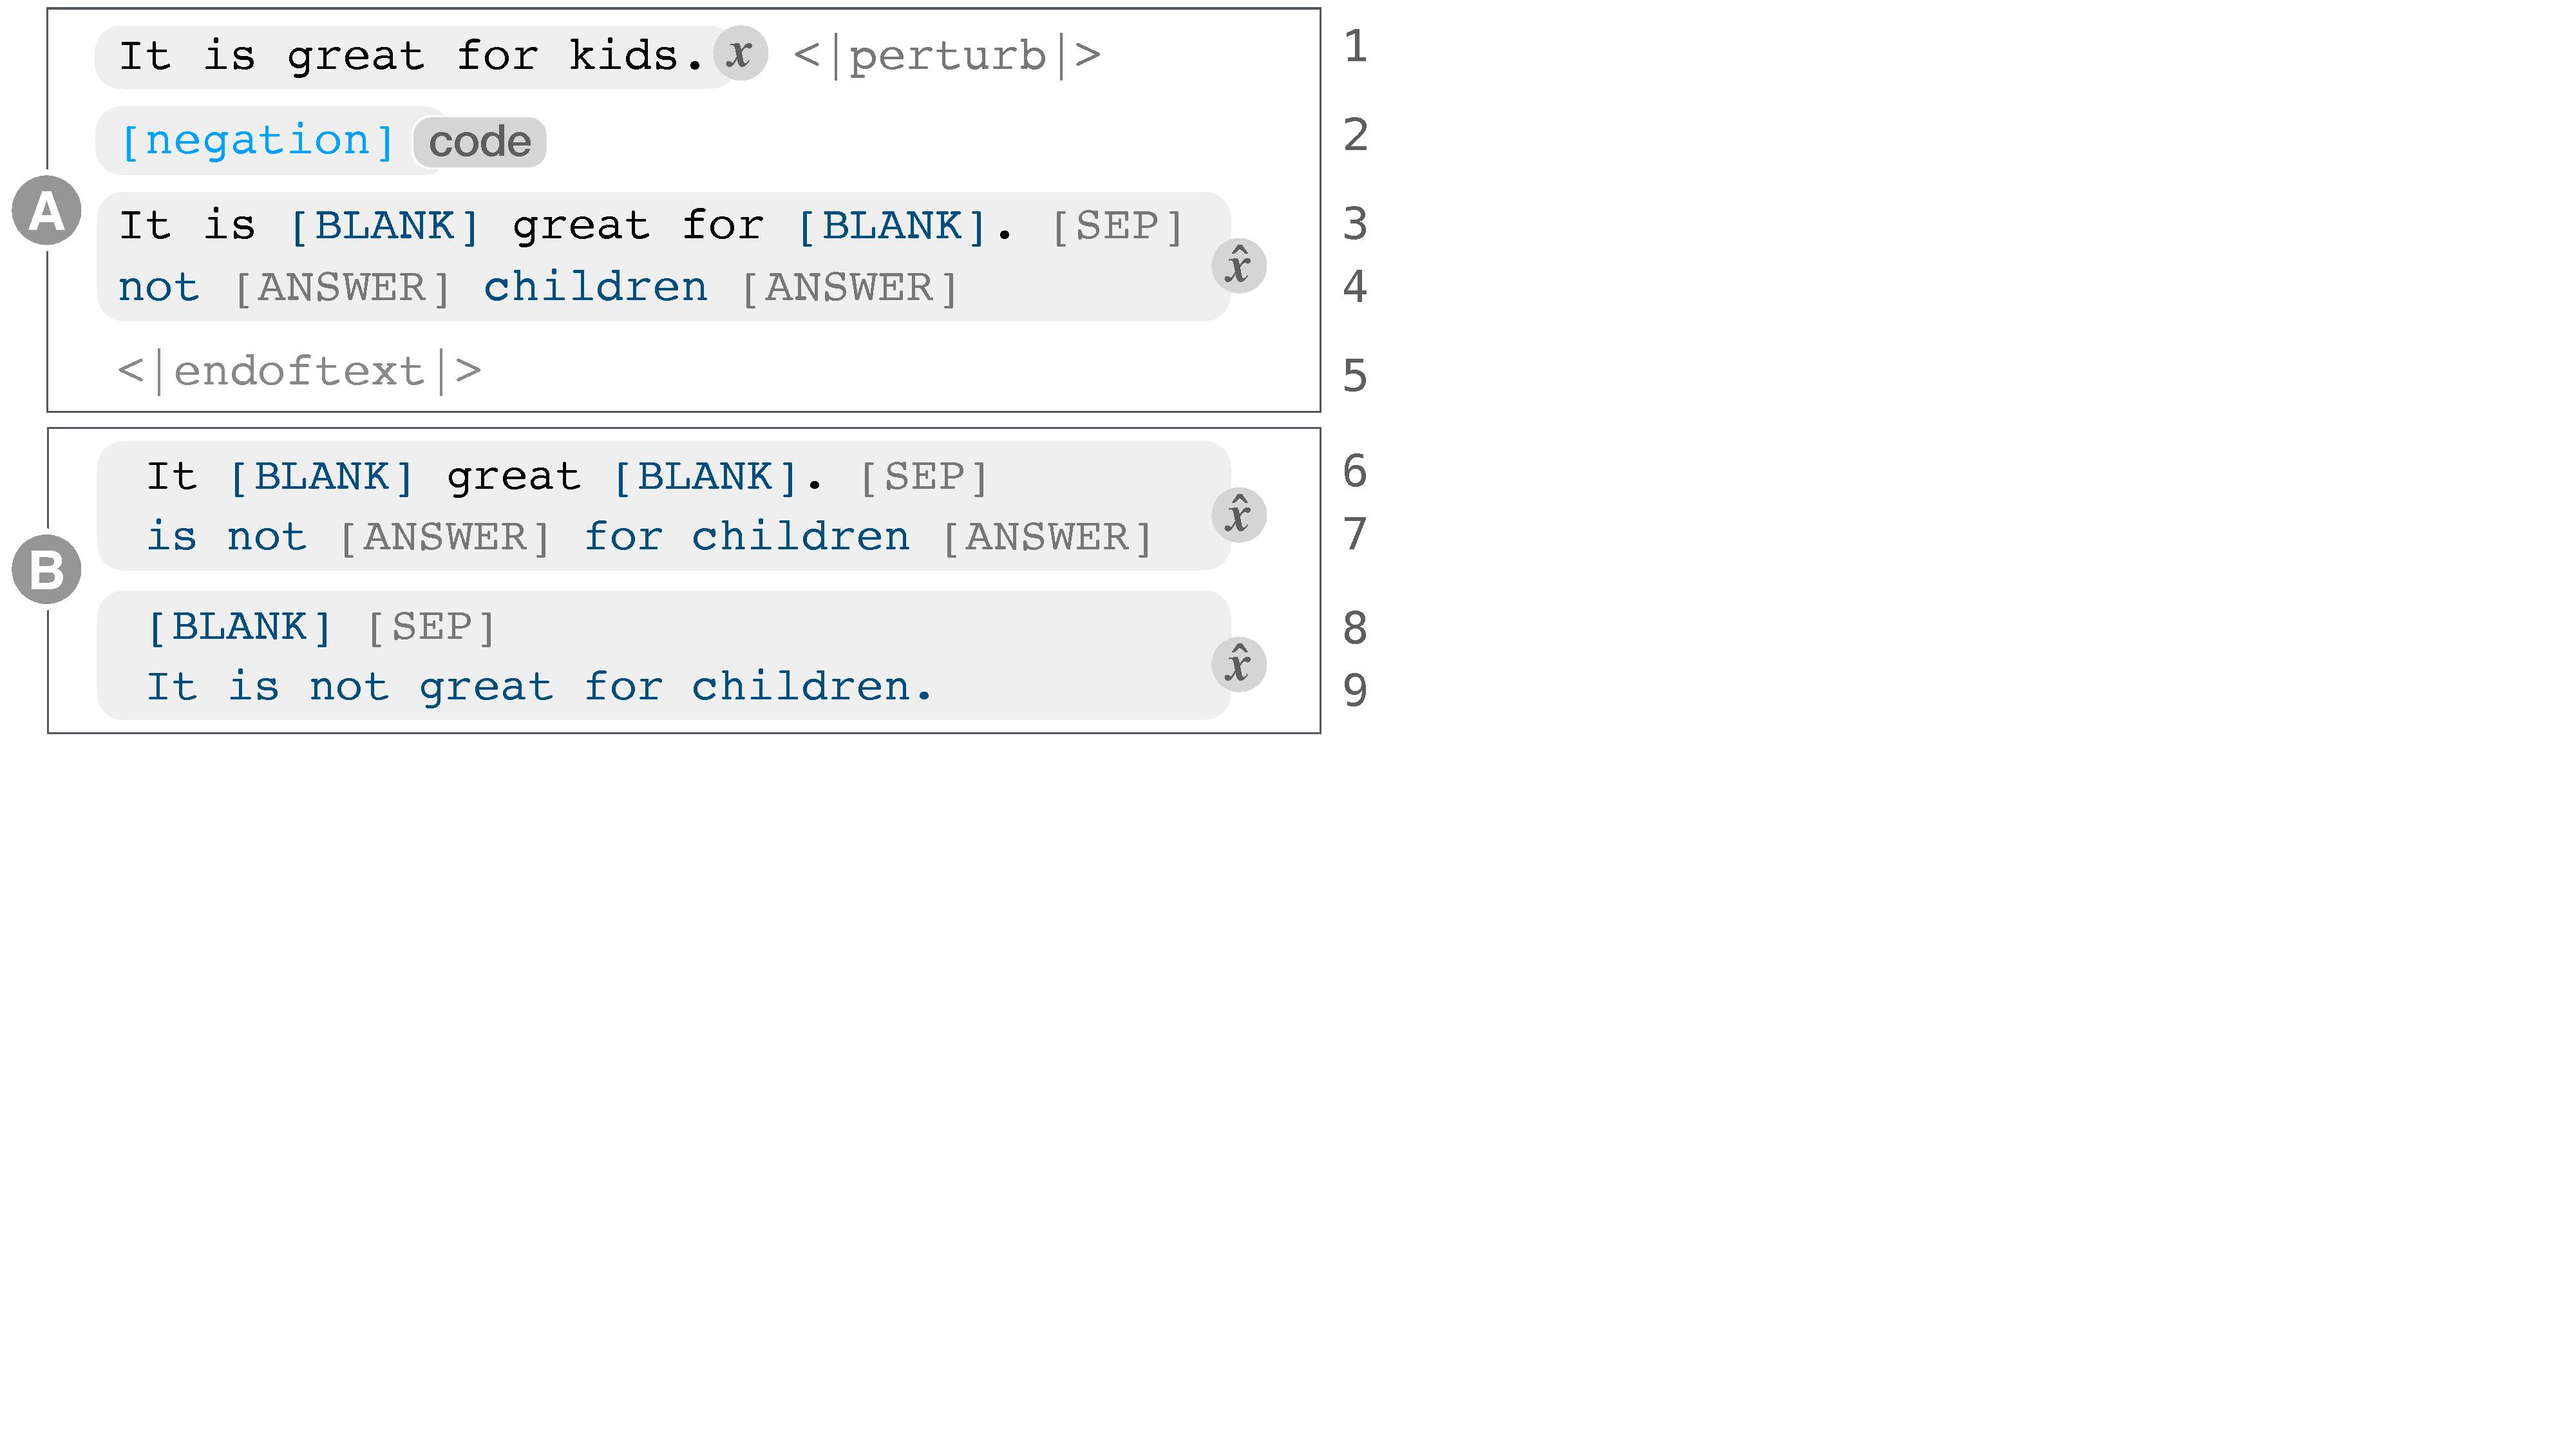
\includegraphics[trim={0 30.7cm 53.2cm 0cm}, clip, width=1\columnwidth]{figures/blank}
\vspace{-15pt}
\caption{Given a pair of sentences $(x, \xp)$, we generate multiple training prompts with (A) a primary \tagstr, and various blanking strategies, from (B) just the changed tokens, (C) the subtrees, (D) the merged changes, and (E) the entire sentence.
%We concatenate the information with special tokens like \perturbtoken.
}
\vspace{-10pt}
\label{fig:blank}
\end{figure}

\subsection{Counterfactual generation as NLG}

We frame the perturbation as a text generation task using language models (LMs), which predict the continuing text given preceding prompts.
%Here, instead of their common use case, \ie generating the remaining paragraphs, 
Pre-trained on a large number of web pages curated and filtered by humans, LMs like GPT-2~\cite{radford2019language} naturally generate more \emph{realistic} and \emph{diverse} counterfactuals compared to templates~\cite{ribeiro2018sear} or perturbation functions~\cite{wu2019errudite}.
We use the original sentence $x$ as the prompt, and finetune off-the-shelf LMs to generate $\xp$: \exinline{$x$ \perturbtoken $\xp$ \stoptoken}.

\paragraph{Training prompts with controls.}
We further modify the training prompts to allow targeted perturbations, as in Figure~\ref{fig:blank}.
Besides boosting diversity on top of LMs, the targeted perturbations enable new forms of downstream applications like interactive explanation~\cite{miller} and slice-based data augmentation~\cite{chen2019slice}.

\emph{Where-to-perturb, with \texttt{[BLANK]}}.
To perturb specific parts of $x$, We borrow the blank fill-in structure~\cite{donahue2020enabling}, \ie targeted subphrases are replaced with special \texttt{[BLANK]} tokens, and the actual content (``answers'' to blanks) are concatenated to the end. 
To allow flexible blanking at the generation time, we extend the blank in training prompts to cover the associated parsing structures of edited spans.
%As a result, we form up to four unique training prompts given one $(x, \xp)$ pair.

\emph{How-to-perturb, with \tagstrs}.
To specify the perturbation strategy, we condition the generation on special \tagstrs (similar to \citet{raffel2019exploring, Dathathri2020Plug}).
The 8 \tagstrs in Table~\ref{table:ctrltag} are summarized from 33 papers on textual counterfactual applications.
We design them to distinguish the information change, with \eg \ctrltag{negation} constraining on concrete behaviors, and \ctrltag{lexical} loosely denoting changes on unigrams or prepositions.
We further maximize the syntactic differences (\eg \ctrltag{resemantic}, \ctrltag{insert}, or \ctrltag{restructure}), such that the controls are more explicit to follow for the model than semantic-oriented ones (synonyms, antonyms, paraphrases).
For a given pair $s(x, \xp)$, we compute the primary \tagstrshort based on linguistic features like part-of-speech tags or dependency trees.
As in Figure~\ref{fig:blank}, we put \tagstrs before the blanked $\xp$ to prioritize \emph{how} over \emph{where}, such that when given a \tagstr, the model can determine the appropriate changing places, and generate the blanked prompt on its own. 
%However, in cases where it is more essential to inspect particular subphrases, it is possible to reverse the order.
%, so we can provide the blanked prompts, and let the model figure out the \emph{how}.
%It is also possible to swap the order of the blanked $\xp$ and the \tagstrs. 

%, we found WordNet~\cite{miller1998wordnet} or sentence similarity based tagging are inaccurate, and the pattern was tricky to learn for the LM model.
%The \tagstrs distinguish the information change: the syntax-preserving ones add (\ctrltag{insert}), remove (\ctrltag{delete}), or change constraints, and the constraints vary from sparse (\ctrltag{resemantic} is more loose than \ctrltag{lexical}) to specific and finer-grained (\ctrltag{negation}, \ctrltag{quantifier}).
%Remaining \ctrltag{shuffle} and \ctrltag{restructure}, on the other hand, focuses on syntactic understanding when we have high lexical overlap.

%\wts{Add some more explanation on the design rationale. It is a more syntactic style change, and we try to minimize the overlaps between words; But we leave out the semantic ones because they overlap too much. arguably lexical and resemantic are similar, but we separate them because editing distance and because too many prior work do lexical change that it deserves a separate category.}

\textbf{Training data formation.}
While we do not have a single training set for counterfactual generation, multiple existing datasets contain pair sentences that can be seen as \emph{close} counterfactuals of each other. 
We combined six such datasets.
They all contain natural sentences (\eg WinoGrande~\cite{sakaguchi2019winogrande} for Commonsense tasks, PAWS~\cite{zhang2019paws} for paraphrasing) such that the finetuned model still maintain \emph{realistic} generation.
Moreover, they each expresses a subset of the strategies, and therefore achieves fair coverage on all \tagstrs when combined.
In total, we collected 657,144 training prompts from 191,415 sentence pairs.
We list the representative datasets in Table~\ref{table:ctrltag}, and describe the datasets and the finetuning details in \S\ref{appendix:train_data}.


\textbf{Filtering \emph{realistic} generations.}
With \tagstrs and blanks,the generated counterfactuals can become ungrammatical or nonsensical, and therefore requires additional filtering.
Inspired by the language model constraints used by \citet{morris2020textattack}, we score both $x$ and $\xp$ using un-finetuned GPT-2, and invalidate the $\xp$ if its log-probability (either on the full sentence or on the perturbed chunks) decreases more than 10 points compared to $x$.
%(though their other constraints may also be useful.)


\textbf{Ranking \& Selection.}
As a general-purpose and task-agnostic model, our generator does not distinguish counterfactual applications.
Rather, it (targetedly) generates a large amount of counterfactuals with different combinations of \tagstrs and blanks, and the generated $\hat{\xset}$ should be further selected or ranked based on the relationship $x \rightarrow \xp$.
For example, we find adversarial examples with common filtering constraints (\eg sentence semantic similarity~\cite{morris2020textattack}).
We demonstrate different selections in \S\ref{sec:app_label} and \S\ref{sec:app_explain}.


%pr["pr_sent"]<=10 and pr["pr_phrase"] <=10
%Perplexity is instantiating; Language modeling as an approximation because it measures real world distribution.




%\& Ablation Studies
\subsection{Intrinsic Evaluations}
\label{subsec:intrinsic}
% random no-pair models. 1142508
%We verify the impact of the filtering and the \tagstrs through human evaluations.
\paragraph{Validity / Realistic.}
We verify the impact of the filtering through human evaluation.
One of the coauthors manually labeled the validity of 600 augmentations generated on 120 instances from the three classification tasks (\sst, \nli, \qqp).
The validity rate among all the generated instances is $61.5\%$, which increases to $78.3\%$ after the filtering. 
As part of the data labeling task in \S\ref{sec:app_label}, we also asked crowdworkers to label whether a perturbed sentence is realistic (\emph{``likely written by a native English speaker''}), and they arrived at similar validation rates ($75.0\%$ for \dsst, $70.0\%$ for \dqqp, and $81.7\%$ for \dnli).
%If no filter at all, the instances you see will only have 60% valid stuff (we care more about precision, every invalid counterfactual shown to a human is wasted time):
%\wts{Maybe no need for the instruction; It's in appendix.}


\paragraph{Controllability.}
We finetune another GPT-2 model with training prompts that \emph{do not} contain the \tagstrshorts (called \emph{\sysname-a}), and quantify the impact of \tagstrs through an ablation study.
For each \tagstr, we compare the \emph{control success rate} of \sysname and \sysname-a on \tofix{250} prompts (from 100 unique original sentences).
For each prompt, we generate counterfactuals through beam search (beam $=10$), and recompute the \tagstrshorts on the top three returns.
We deem the control successful if at least one of the three recomputed \tagstrshort matches the input (though in \sysname-a, we only measure whether the \tagstrshort naturally occurs in the uncontrolled generation.)
The success rate increases by $28.4\% \pm 18.2\%$ across all \tagstrs, ranging from \ctrltag{quantifier} (increasing 8\%, from 40.4\% to 48.4\%) to \ctrltag{insert} (64.1\%, from 13.5\% to 78.6\%).
%\ctrltag{lexical} has the smallest increment \tofix{from $93\%$ to $100\%$}, mostly because \emph{\sysname-a} tend to frequently replace words.
%\ctrltag{insert} is the most impactful \tagstrshort (from \tofix{$12\%$ to $100\%$}) --- \sysname-a rarely insert additional clues on its own.

There are three common failure cases for the \tagstrshorts:
%Note that all the prompts used are guaranteed to allow the corresponding \tagstrs, and the \tagstrshorts can be less effective on more general prompts:
(1) The dual manipulation from the \tagstrs and the blanks are in conflict, \eg \exinline{a dog is embraced by a \texttt{[BLANK]}} would not respond to \ctrltag{negation}.
(2) $x$ does not have the corresponding pattern. \ctrltag{shuffle} is not applicable when the sentence has only one adjective or noun (\eg \exinline{the movie is good}).
(3) Certain pattern is very prominent that it dominates the generation probability, \eg the model tends to perturb the quantifier ``two'' in \exinline{two dogs are running}, regardless of the \tagstrshort.
In the ablation study, we filtered out prompts that fell under cases 1 and 2.





